\chapter{Исследовательская часть}

\section{Технические характеристики}
Характеристики используемого оборудования:
\begin{itemize}
    \item[---] Операционная система --- Windows 11 Home \cite{windows}
    \item[---] Память --- 16 Гб.
    \item[---] Процессор --- 12th Gen Intel(R) Core(TM) i7-12700H @  2.30 ГГц \cite{intel}
    \item[---] Микроконтроллер --- STM32F303 \cite{stm}
\end{itemize}

\section{Описание используемых типов данных}
Используемые типы данных:

размер матрицы --- целое число типа $size\_t$;

матрица --- $double **$.

\clearpage

\section{Время выполнения алгоритмов}
Результаты замеров времени работы трех алгоритмов умножения матриц приведены в таблице \ref{tbl:time_mes}. Время работы замерялось на микроконтроллере $STM32F303$ с тактовой частотой до 72 Мгц. Замеры времени проводились на матрицах одинаковой длины и усреднялись для каждого набора одинаковых экспериментов. Каждое значение получено путем взятия среднего из 100 измерений. Зависимости времени умножения от размера матрицы для трех алгоритмов представлены на рисунке \ref{fig:time_mes}.

\begin{table}[h]
    \begin{center}
        \begin{threeparttable}
            \captionsetup{justification=raggedright,singlelinecheck=off}
            \caption{Время работы алгоритмов (в мс)}
            \label{tbl:time_mes}
            \begin{tabular}{|r|r|r|r|}
                \hline
                Размер матрицы & Классический & Виноград & Виноград (оптимизированный) \\
                \hline
                0  & 0.00  & 0.23  & 0.00  \\
                \hline
                2  & 0.24  & 0.52  & 0.18  \\
                \hline
                4  & 1.03  & 0.74  & 1.48  \\
                \hline
                6  & 2.07  & 3.14  & 2.51  \\
                \hline
                8  & 4.56  & 5.67  & 4.72  \\
                \hline
                10 & 7.82  & 9.13  & 8.24  \\
                \hline
                12 & 14.07 & 14.62 & 13.57 \\
                \hline
                14 & 22.49 & 23.21 & 21.08 \\
                \hline
                16 & 30.13 & 34.95 & 28.37 \\
                \hline
                18 & 50.48 & 48.33 & 39.58 \\
                \hline
                20 & 60.72 & 65.83 & 54.97 \\
                \hline
                22 & 85.34 & 82.19 & 74.23 \\
                \hline
                24 & 110.27 & 107.89 & 98.64 \\
                \hline
                26 & 140.12 & 135.48 & 125.32 \\
                \hline
                28 & 174.68 & 170.57 & 154.98 \\
                \hline
                30 & 215.32 & 205.86 & 195.47 \\
                \hline
                32 & 260.59 & 245.32 & 230.14 \\
                \hline
                34 & 320.13 & 290.68 & 275.79 \\
                \hline
                36 & 375.72 & 350.21 & 330.48 \\
                \hline
                38 & 440.65 & 405.34 & 380.73 \\
                \hline
                40 & 510.48 & 475.27 & 450.32 \\
                \hline
                42 & 590.23 & 540.19 & 510.87 \\
                \hline
                44 & 680.79 & 620.35 & 600.24 \\
                \hline
                46 & 790.41 & 710.74 & 690.68 \\
                \hline
                48 & 910.52 & 810.59 & 780.13 \\
                \hline
                50 & 1040.19 & 930.48 & 870.77 \\
                \hline
            \end{tabular}
        \end{threeparttable}
    \end{center}
\end{table}

\begin{figure}[H]
    \centering
    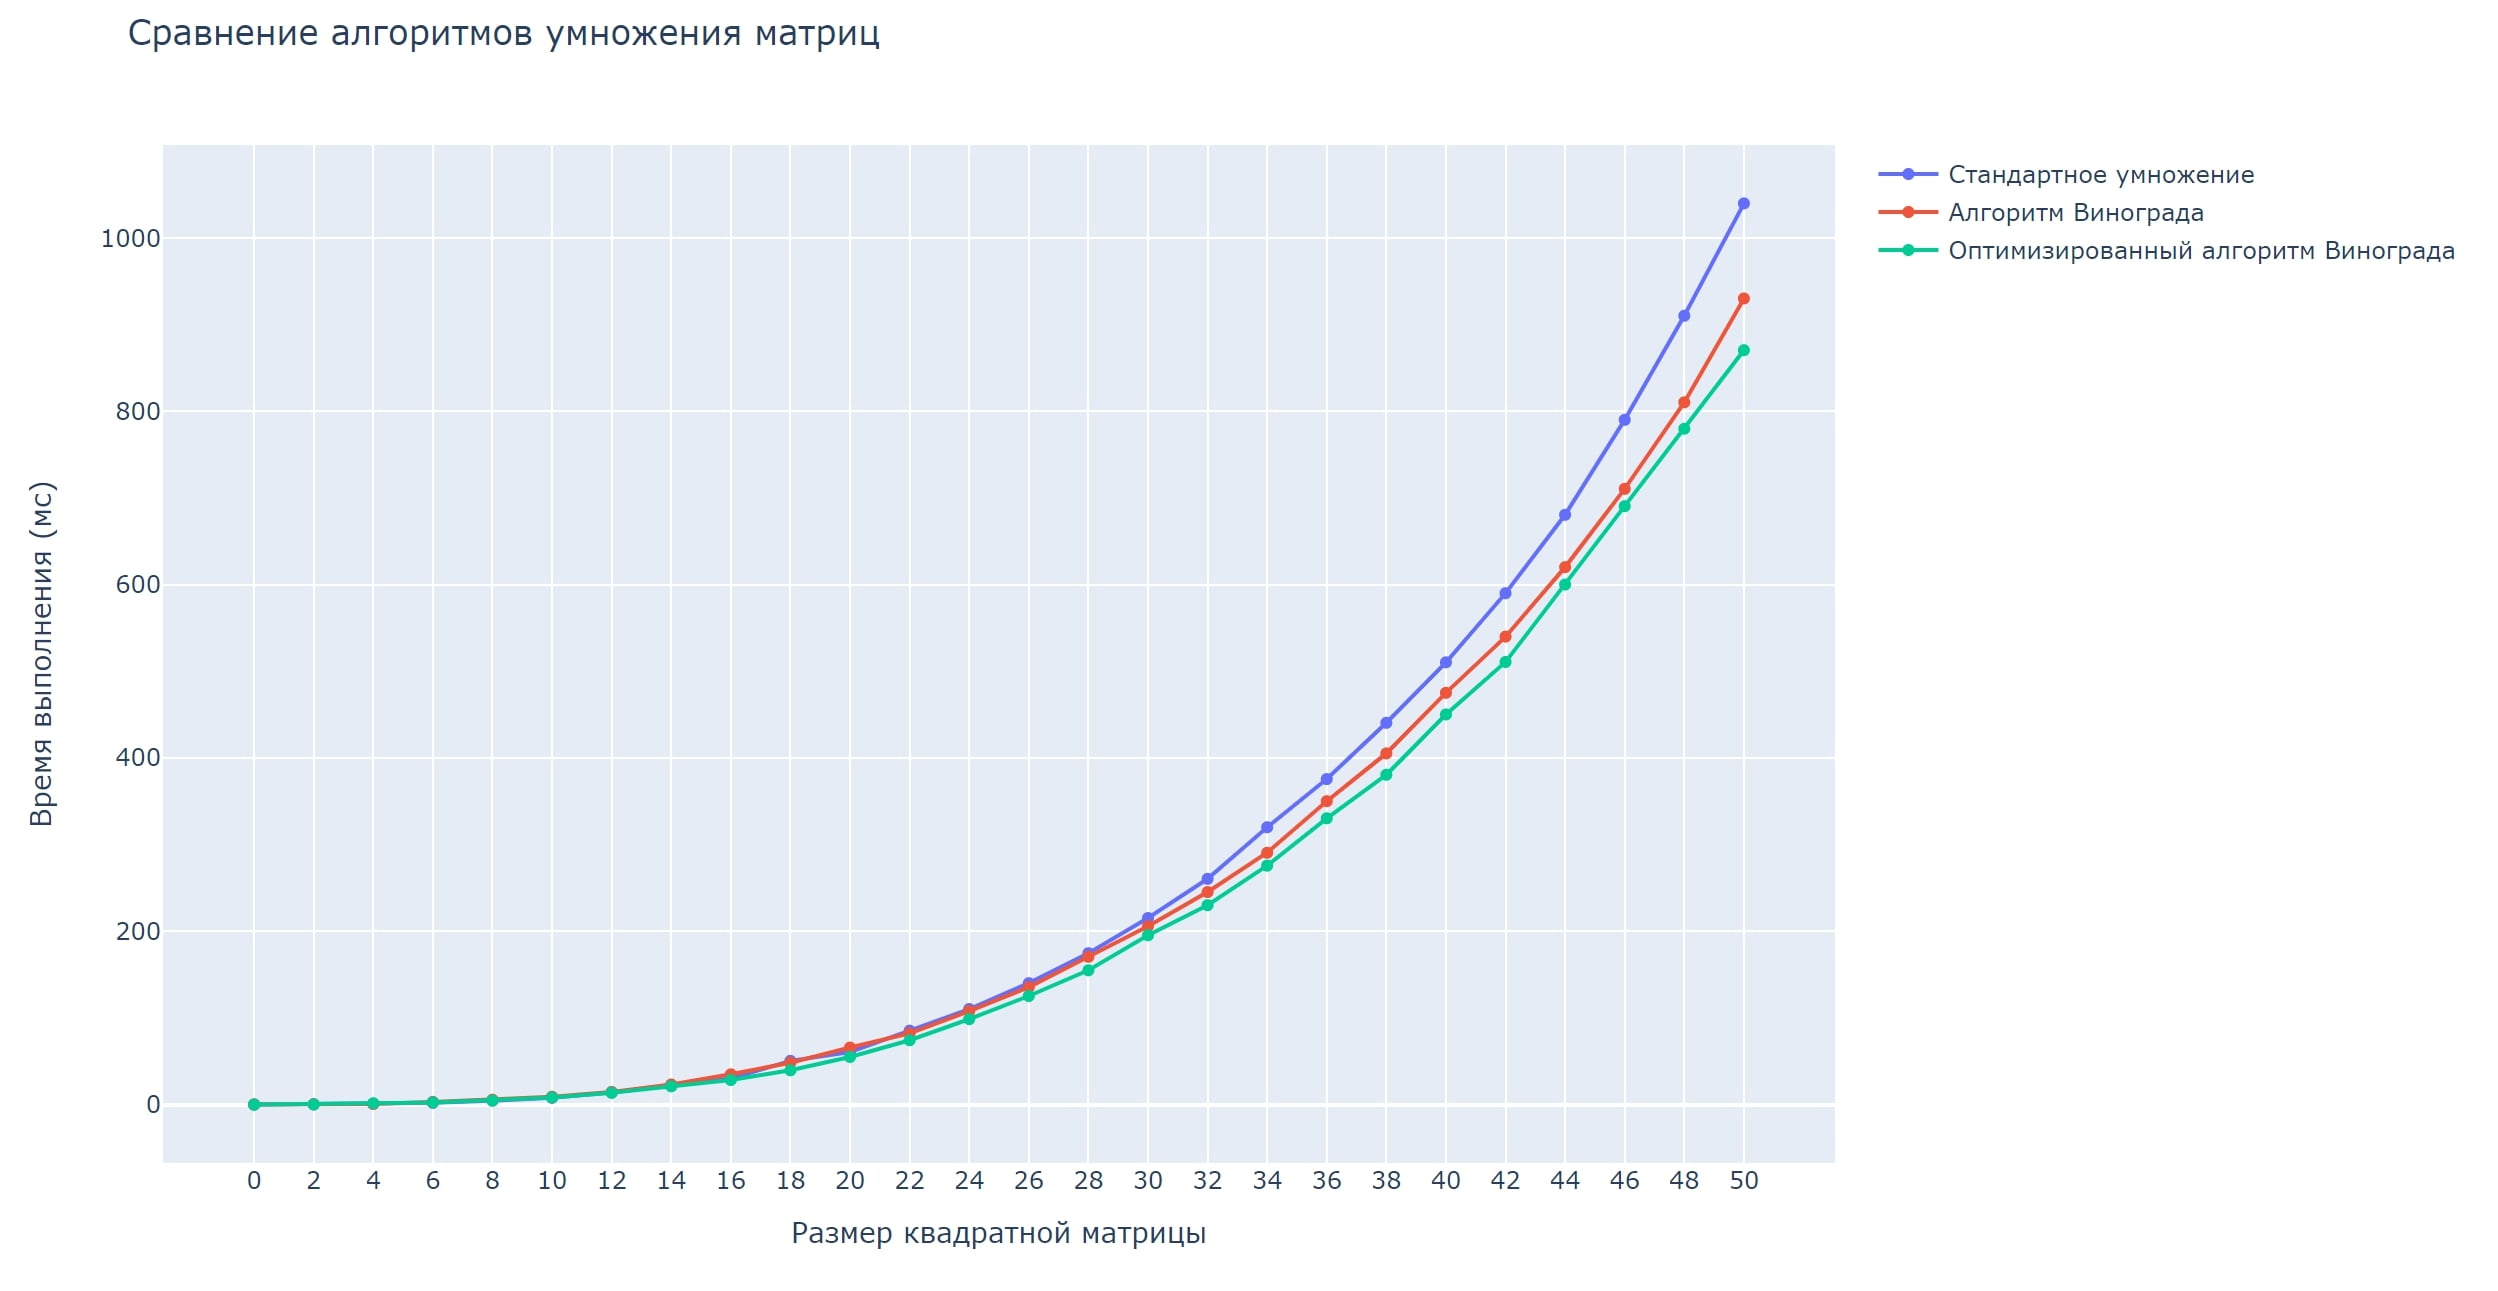
\includegraphics[width=1\linewidth]{images/plots/plot.jpg}
    \caption{Сравнение алгоритмов по времени}
    \label{fig:time_mes}
\end{figure}

\clearpage

\section{Вывод}

В ходе исследования установлено, что для больших размеров матриц (более 10) алгоритм Винограда оказывается более чем в 1.2 раза быстрее классического алгоритма, а оптимизированная версия алгоритма Винограда превосходит стандартный алгоритм почти в 1.3 раза. Это позволяет заключить, что для таких данных наиболее целесообразно применять оптимизированный алгоритм Винограда.

Также было выявлено, что алгоритм Винограда работает эффективнее на матрицах с четными размерами, поскольку для нечетных матриц требуются дополнительные вычисления для обработки крайних строк и столбцов. Таким образом, алгоритм Винограда рекомендуется использовать при работе с матрицами четных размеров.